\documentclass[12pt,letterpaper]{article}
\usepackage[utf8]{inputenc}
\usepackage[spanish]{babel}
\usepackage{graphicx}
\usepackage[left=2cm,right=2cm,top=2cm,bottom=2cm]{geometry}
\usepackage{graphicx} % figuras
% \usepackage{subfigure} % subfiguras
\usepackage{float} % para usar [H]
\usepackage{amsmath}
%\usepackage{txfonts}
\usepackage{stackrel} 
\usepackage{multirow}
\usepackage{enumerate} % enumerados
\renewcommand{\labelitemi}{$-$}
\renewcommand{\labelitemii}{$\cdot$}
% \author{}
% \title{Caratula}
\begin{document}

% Fancy Header and Footer
% \usepackage{fancyhdr}
% \pagestyle{fancy}
% \cfoot{}
% \rfoot{\thepage}
%

% \usepackage[hidelinks]{hyperref} % CREA HYPERVINCULOS EN INDICE

% \author{}
\title{Caratula}

\begin{titlepage}
\begin{center}
\large{UNIVERSIDAD PRIVADA DE TACNA}\\
\vspace*{-0.025in}
\begin{figure}[htb]
\begin{center}

\includegraphics[width=8cm]{./Imagenes/logo}
\end{center}
\end{figure}
\vspace*{0.15in}
INGENIERIA DE SISTEMAS  \\

\vspace*{0.5in}
\begin{large}
TITULO:\\
\end{large}

\vspace*{0.1in}
\begin{Large}
\textbf{Informe Laboratorio N° 02 } \\
\end{Large}

\vspace*{0.3in}
\begin{Large}
\textbf{CURSO:} \\
\end{Large}

\vspace*{0.1in}
\begin{large}
INTELIGENCIA DE NEGOCIOS\\
\end{large}

\vspace*{0.3in}
\begin{Large}
\textbf{DOCENTE(ING):} \\
\end{Large}

\vspace*{0.1in}
\begin{large}
 Patrick Cuadros Quiroga\\
\end{large}

\vspace*{0.2in}
\vspace*{0.1in}
\begin{large}
Integrantes: \\
\begin{flushleft}
Merino Quispe, Katerin Almendra 	\hfill	(2018060918) \\
\end{flushleft}
\end{large}
\end{center}

\end{titlepage}


\tableofcontents % INDICE
\thispagestyle{empty} % INDICE SIN NUMERO
\newpage
\setcounter{page}{1} % REINICIAR CONTADOR DE PAGINAS DESPUES DEL INDICE

\begin{center}
    PRACTICA DE LABORATORIO N° 02
\end{center}

\section{OBJETIVOS}
Crear relaciones automáticas y manuales

\section{REQUERIMIENTOS}

\begin{itemize}

\item Conocimientos
\\Para el desarrollo de esta práctica se requerirá de los siguientes conocimientos básicos:
\\- Conocimientos básicos de administración de base de datos Microsoft SQL Server.
\\- Conocimientos básicos de SQL.
\item Software
\\Asimismo se necesita los siguientes aplicativos:
\\- Microsoft SQL Server 2016 o superior
\\- Base de datos AdventureWorks2016 o superior
\\- Power BI Desktop.
\\- Tener una cuenta Microsoft registrada en el Portal de Power Bi
\end{itemize}

\section{CONSIDERACIONES INICIALES}
\item Generar una carpeta o directorio Power BI en un lugar accesible para guardar los resultados de la práctica.

\section{DESARROLLO} 
\section*{Ejercicio 1: Crear relaciones}
\item \textbf{Tarea 1: Relaciones automáticas}
\begin{itemize}
\item  1. Ingresar a Power BI Desktop.
\item  2. En la Ventana de Power BI Desktop, click en Obtener Datos (Get Data)
\item  3. En el cuadro de dialogo Obtener Datos (Get Data), asegurarse que Excel esta seleccionado y hacer click en Conectar (Connect).
\end{itemize} 

\begin{center}
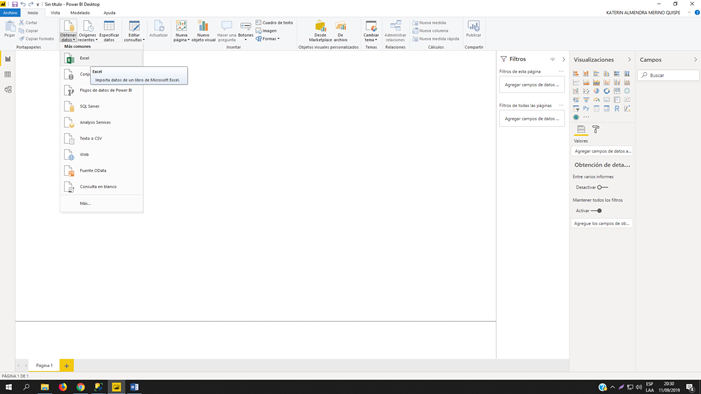
\includegraphics[width=15cm]{./Imagenes/img01} 
\end{center}

\begin{itemize}
\\ 4. En el cuadro de dialogo Abrir (Open), buscar el archivo Adventure Works Sales Data.xlsx, y luego hacer click en Abrir (Open).
\end{itemize} 

\begin{center}
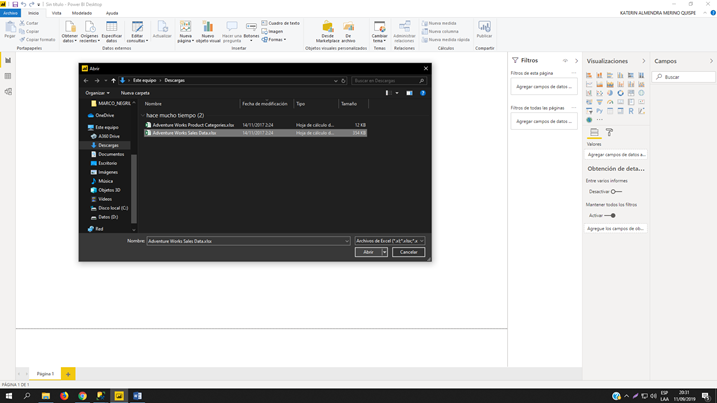
\includegraphics[width=15cm]{./Imagenes/img02} 
\end{center}

\begin{itemize}
\\ 5. En el cuadro de dialogo Explorador (Navigator), seleccionar las hojas DimCurrency, DimCustomer,
DimDate, DimProduct, DimPromotion, DimSalesTerritory, y FactInternetSales.
\\ 6. Hacer click en Cargar (Load).

\end{itemize} 

\begin{center}
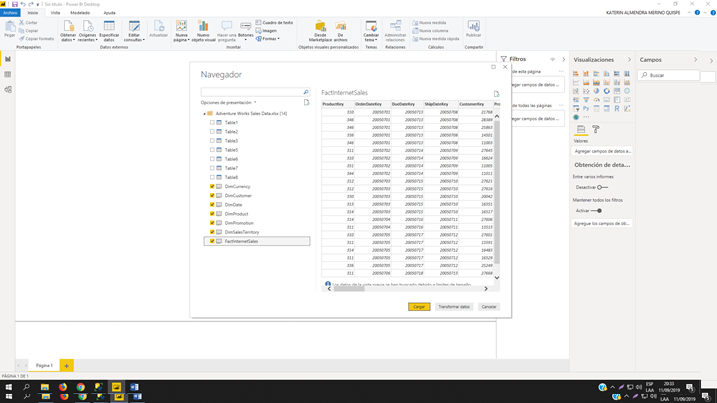
\includegraphics[width=15cm]{./Imagenes/img03} 
\end{center}

\item 7. En el panel de vistas a mano derecho, hacer click en Relaciones (Relationships).
\item 8. En el menú principal, hacer click en Administrar relaciones (Manage Relationships).
\begin{center}
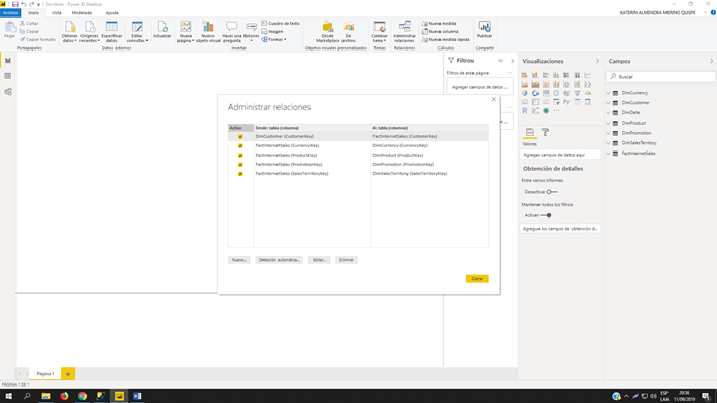
\includegraphics[width=15cm]{./Imagenes/img04} 
\end{center}


\begin{itemize}
\item 9. En el cuadro de Administrar relaciones (Manage Relationships), hacer click en Nueva (New)
\end{itemize}

\begin{center}
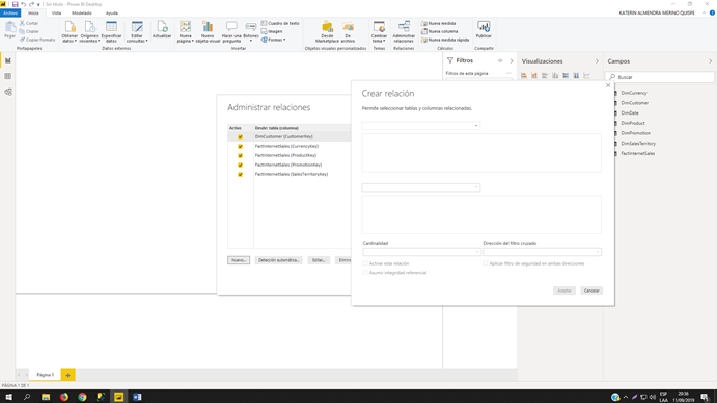
\includegraphics[width=15cm]{./Imagenes/img05} 
\end{center}

\item 10. En el cuadro de Administrar relaciones (Manage Relationships), en la lista de tablas superior, hacer click en FactInternetSales. Cuando la vista previa de la table aparezca hacer click en la columna
OrderDateKey.

\begin{center}
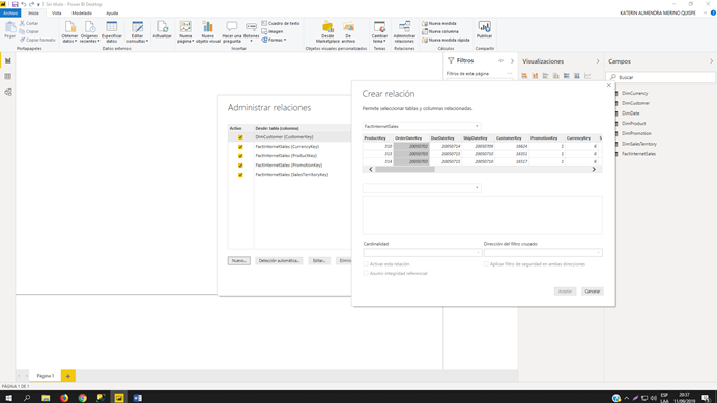
\includegraphics[width=15cm]{./Imagenes/img06} 
\end{center}

\item 11. En la lista de table inferior, hacer click en DimDate. Cuando la vista previa de la table aparezca hacer click en la columna DateKey. 

\begin{center}
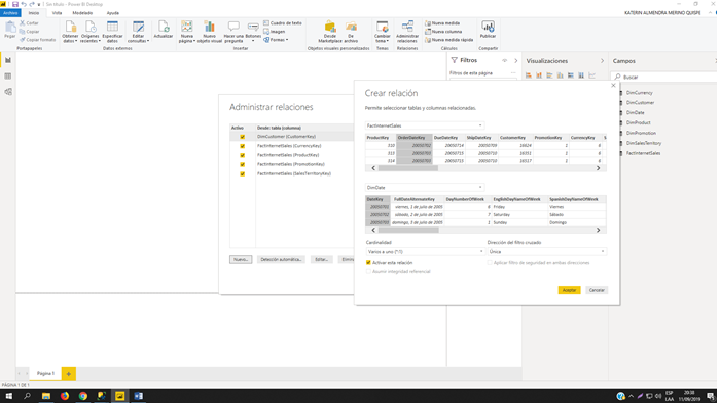
\includegraphics[width=15cm]{./Imagenes/img07} 
\end{center}

\item 12. Revisar que la cardinalidad (Cardinality) esta seleccionada para Muchos a Uno (Many to One (*:1)), que la Dirección del filtro cruzado (Cross filter direction) es Sencilla (Single), y que la opción Hacer esta relación activa (Make this relationship active) se encuentra seleccionada, luego hacer click en Aceptar (OK).
\item 13. En el cuadro de Administrar relaciones (Manage Relationships), hacer click en Cerrar (Close).

\begin{center}
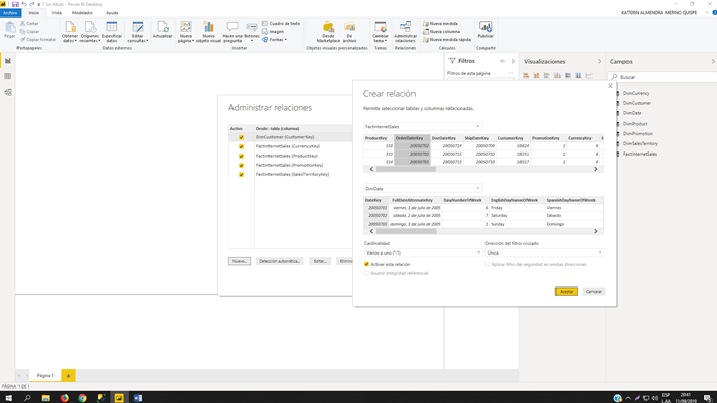
\includegraphics[width=15cm]{./Imagenes/img08} 
\end{center}

\item 14. En el diagrama, en la tabla FactInternetSales, hacer click en la columna DueDateKey. Arrastrar la columna DueDateKey a la columna DateKey de la tabla DimDate.

\item 15. En el diagrama, en la tabla FactInternetSales, hacer click en la columna ShipDateKey. Arrastrar la columna ShipDateKey a la columna DateKey de la tabla DimDate.

\begin{center}
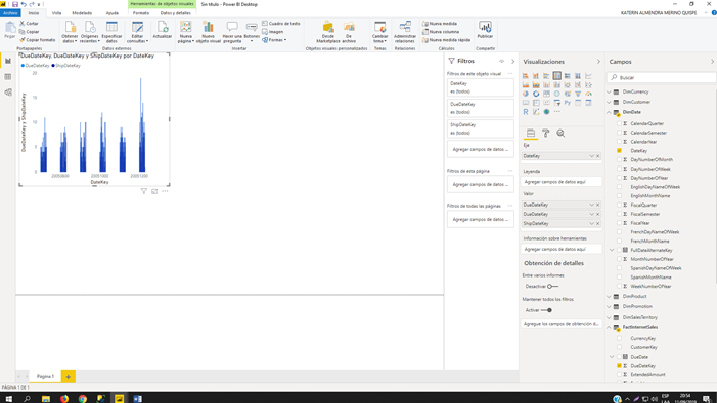
\includegraphics[width=15cm]{./Imagenes/img09} 
\end{center}
\item 16. En el menú principal, hacer click en Administrar relaciones (Manage Relationships).
\item 17. En el cuadro de Administrar relaciones (Manage Relationships), hacer doble click en la relación
FactInternetSales (CurrencyKey).
\item 18. En la lista de Dirección de Filtro Cruzado (Cross filter direction), hacer click en Sencilla (Single), luego hacer click en Aceptar (OK).
\begin{center}
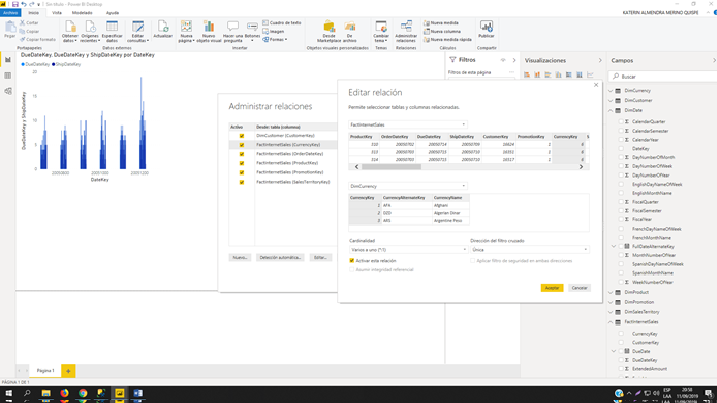
\includegraphics[width=15cm]{./Imagenes/img10} 
\end{center}
\item 19. En el cuadro de Administrar relaciones (Manage Relationships), hacer doble click en la relación
FactInternetSales (ProductKey).
\item 20. En la lista de Dirección de Filtro Cruzado (Cross filter direction), hacer click en Sencilla (Single), luego hacer click en Aceptar (OK). 

\begin{center}
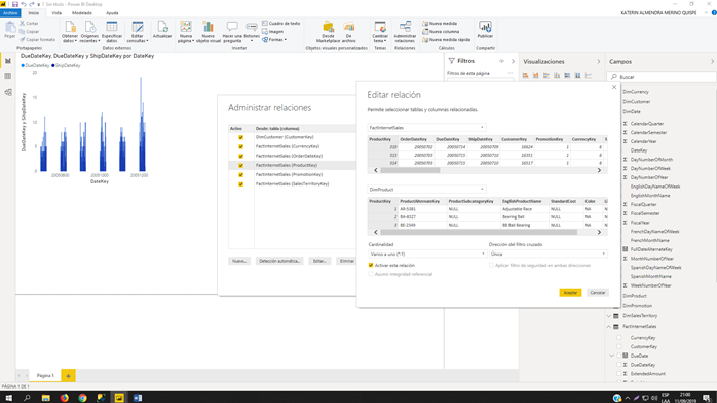
\includegraphics[width=15cm]{./Imagenes/img11} 
\end{center}
\item 21. En el cuadro de Administrar relaciones (Manage Relationships), hacer doble click en la relación
FactInternetSales (PromotionKey).
\item 22. En la lista de Dirección de Filtro Cruzado (Cross filter direction), hacer click en Sencilla (Single), luego hacer click en Aceptar (OK)

\begin{center}
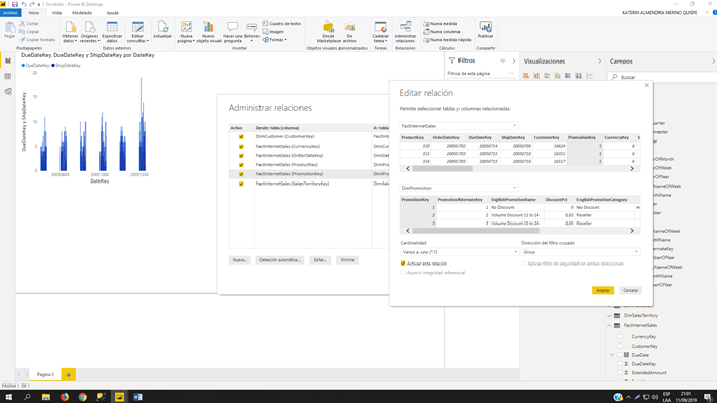
\includegraphics[width=15cm]{./Imagenes/img12} 
\end{center}
\item 23. En el cuadro de Administrar relaciones (Manage Relationships), hacer doble click en la relación
FactInternetSales (SalesTerritoryKey).
\item 24. En la lista de Dirección de Filtro Cruzado (Cross filter direction), hacer click en Sencilla (Single), luego hacer click en Aceptar (OK). 

\begin{center}
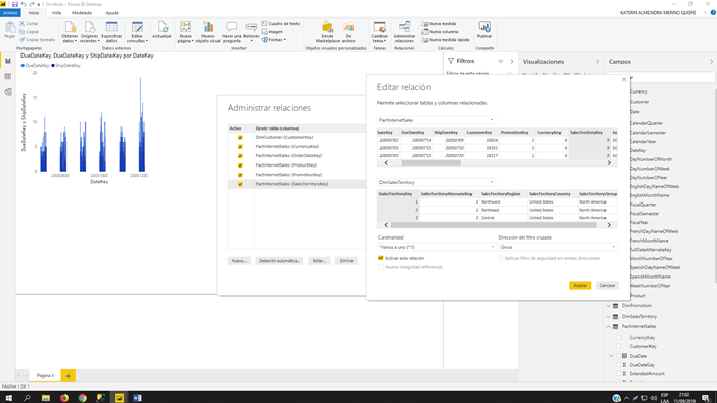
\includegraphics[width=15cm]{./Imagenes/img13} 
\end{center}

\item 25. En el cuadro de Administrar relaciones (Manage Relationships), hacer click en Cerrar (Close)..

\begin{center}
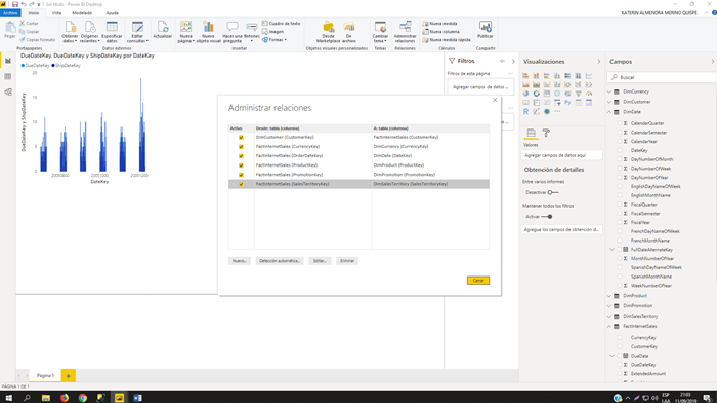
\includegraphics[width=15cm]{./Imagenes/img14} 
\end{center}
\item 26. Hacer click en la línea de relación entre FactInternetSales and DimCustomer y presionar Borrar (Delete).
\item 27. En el cuadro de dialogo Eliminar relación (Delete Relationship), hacer click en Borrar (Delete).

\begin{center}
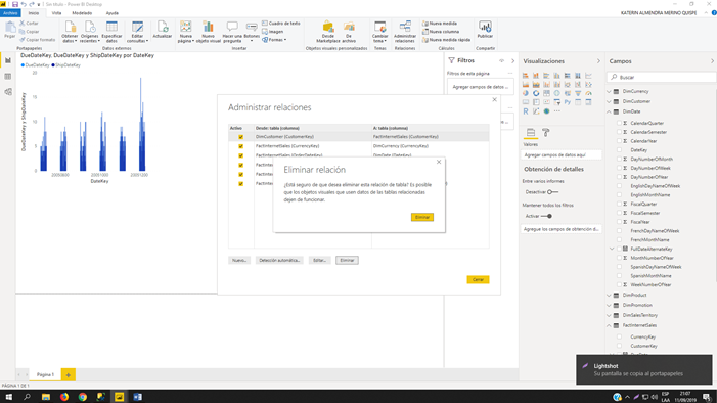
\includegraphics[width=15cm]{./Imagenes/img15} 
\end{center}
\item 28. En el menú principal, hacer click en Administrar relaciones (Manage Relationships).
\item 29. En el cuadro de Administrar relaciones (Manage Relationships), hacer click en Nueva (New).
\item 30. En la lista de tablas superior, hacer click en FactInternetSales. Luego hacer click en la columna CustomerKey en la vista de datos previa.
\item 31. En la lista de tablas superior, hacer click en DimCustomer, y hacer click CustomerKey en la vista de datos previa.
\item 32. En la lista de Cardinalidad (Cardinality), hacer click en Muchos a Uno (Many to One (*:1)), y luego hacer click en Aceptar (OK).

\begin{center}
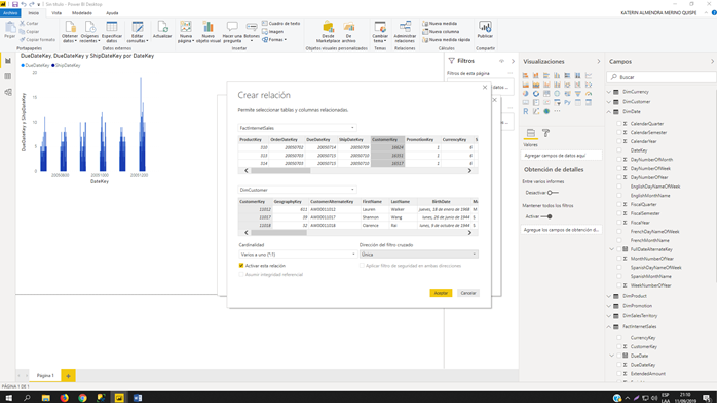
\includegraphics[width=15cm]{./Imagenes/img16} 
\end{center}

\item 33. En el cuadro de Administrar relaciones (Manage Relationships), hacer click en Cerrar (Close).
\item 34. Hacer click en Guardar (Save), y cuargar el archive como Ventas Adventure Works.pbix. 
\begin{center}
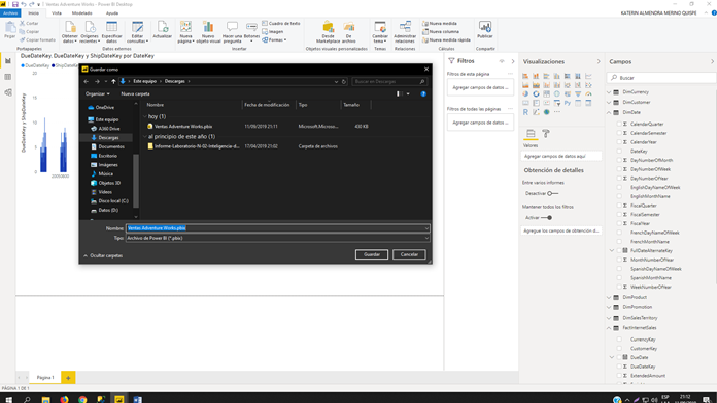
\includegraphics[width=15cm]{./Imagenes/img17} 
\end{center}
\\\\
\item \textbf{Tarea 2: Relaciones manuales}

\item 1. En la Ventana de Power BI Desktop, click en Obtener Datos (Get Data) y luego en Excel
\item 2. Abrir el archivo Adventure Works Product Categories.xlsx.

\begin{center}
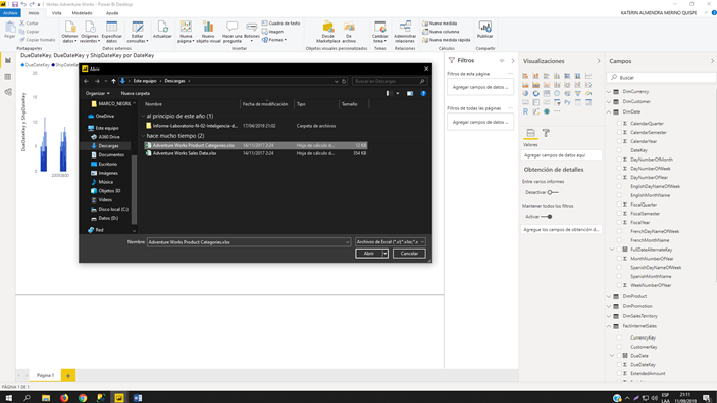
\includegraphics[width=15cm]{./Imagenes/img18} 
\end{center}

\item 3. En el cuadro de dialogo Explorador (Navigator), seleccionar las hojas DimProductCategory, and
DimProductSubcategory, y luego hacer click en Cargar (Load).

\begin{center}
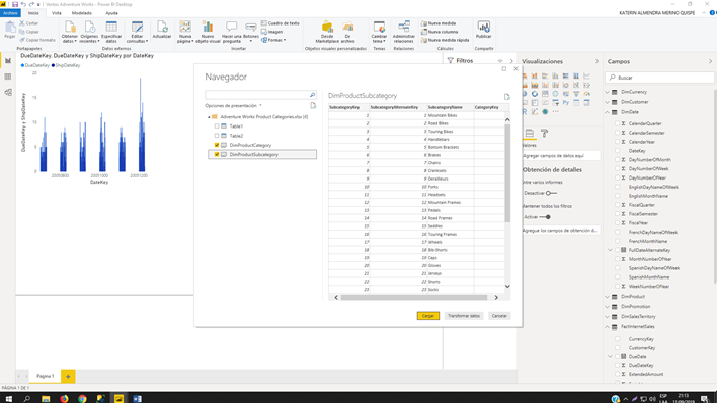
\includegraphics[width=15cm]{./Imagenes/img19} 
\end{center}

\item 4. En el panel de Relaciones, revisar la relación que Power BI ha creado entre las dos tablas.
\item 5. Hacer click en la línea de la relación entre DimProductCategory, y DimProductSubcategory, y seleccionar Eliminar (Delete).
\item 6. En el cuadro de dialogo Eliminar relación (Delete Relationship), hacer click en Borrar (Delete).

\begin{center}
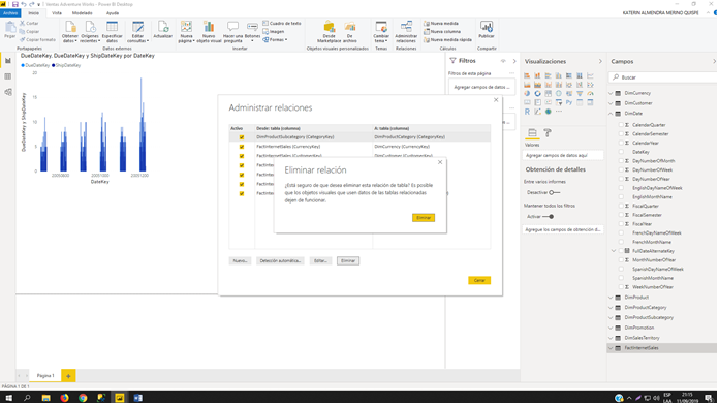
\includegraphics[width=15cm]{./Imagenes/img20} 
\end{center}

\item 7. Arrastrar la columna CategoryKey en la tabla DimProductSubcategory a la columna Category en la tabla DimProductCategory, para crear una relación Muchos a uno (Many to One (*:1)), y una dirección de filtro cruzado (Cross filter direction) en ambos
\begin{center}
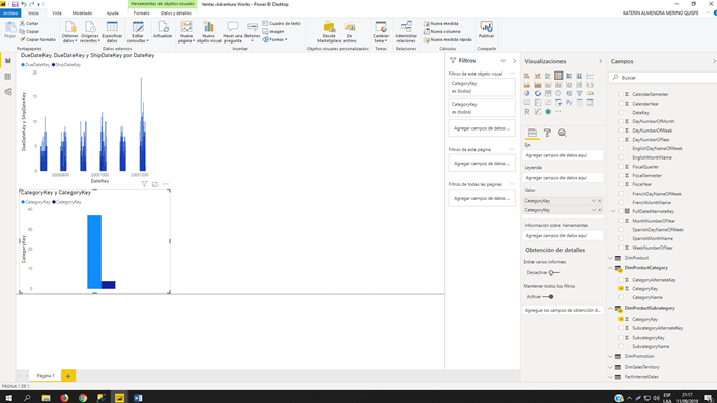
\includegraphics[width=15cm]{./Imagenes/img21} 
\end{center}

\item 8. En la tabla DimProduct, arrastrar la columna ProductSubcategoryKey a la columna SubcategoryKey en la tabla DimProductSubcategory, para crear una relación de Muchos a Uno (Many to One (*:1)), y una dirección de filtro cruzado (Cross filter direction) en ambos.
\begin{center}
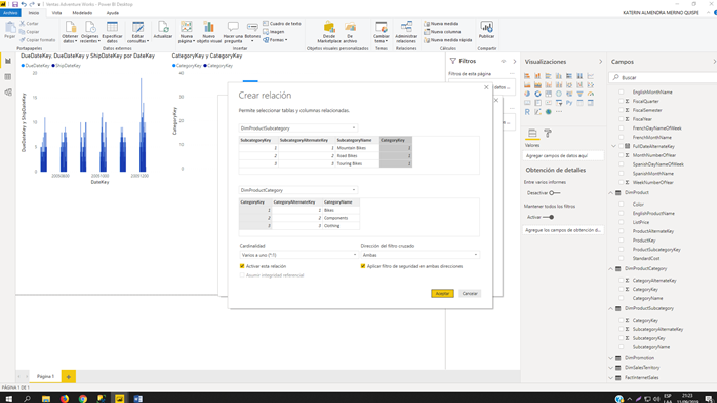
\includegraphics[width=15cm]{./Imagenes/img22} 
\end{center}

\item 9. Hacer click en Guardar

\section*{Ejercicio 2: Cálculos}
\item \textbf{Tarea 1: Add a Calculated Column}

\item 1. In Power BI Desktop, click Data in the views pane on the left-hand side.
\item 2. In the Fields pane, click DimCustomer.
\item 3. On the Modeling ribbon, in the Calculations group, click New Column.
\item 4. In the formula bar, highlight Column =, and type:
IncomeStatus = IF (DimCustomer[YearlyIncome] < 25000, "Lower Income",
IF (AND(DimCustomer[YearlyIncome] >= 25000, DimCustomer[YearlyIncome] < 60000),
"Middle Income",
IF (AND(DimCustomer[YearlyIncome] >= 60000, DimCustomer[YearlyIncome] < 100000),
"Higher Income",
IF (DimCustomer[YearlyIncome] >= 100000, "Very High Income", "Other"))))
\item 5. Press Enter.


\begin{center}
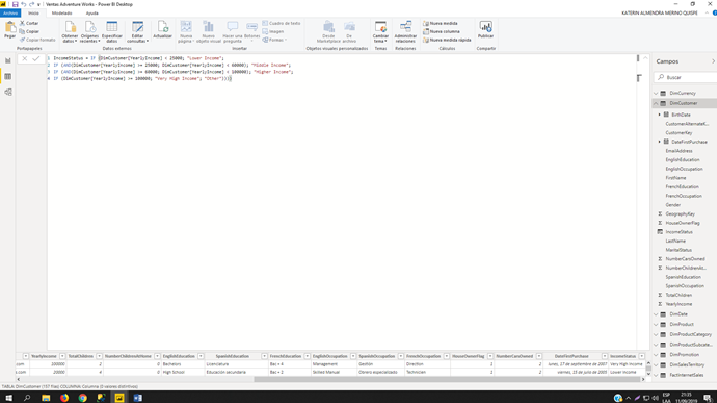
\includegraphics[width=15cm]{./Imagenes/img23} 
\end{center}

\begin{center}
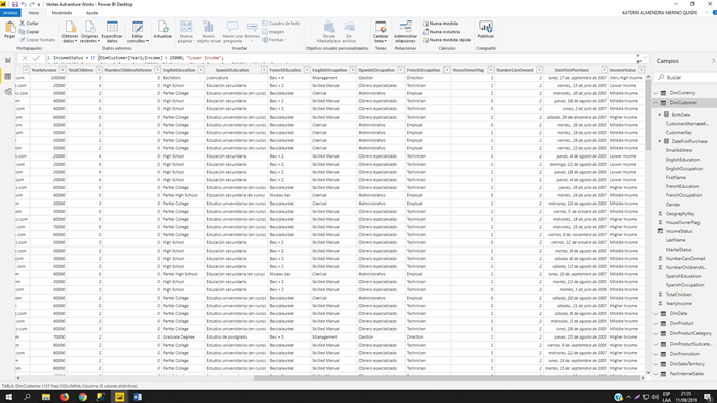
\includegraphics[width=15cm]{./Imagenes/img24} 
\end{center}

\item 6. On the Modeling ribbon, in the Calculations group, click New Column.
\item 7. In the formula bar, highlight Column =, and type:
DaysSinceFirstPurchase = DATEDIFF(DimCustomer[DateFirstPurchase], TODAY(), DAY)
\item 8. Press Enter. 
\begin{center}
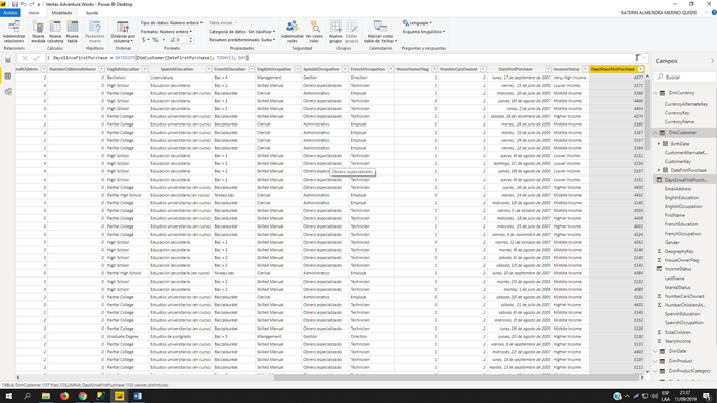
\includegraphics[width=15cm]{./Imagenes/img25} 
\end{center}

\item 9. On the Modeling ribbon, in the Calculations group, click New Column.
\item 10. In the formula bar, highlight Column =, and type:
FullName = [FirstName] & " " & [LastName]
\item 11. Press Enter.
\begin{center}
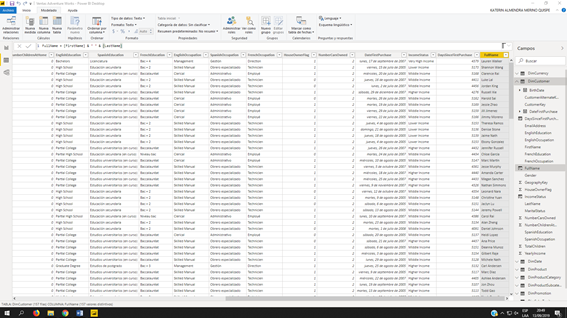
\includegraphics[width=15cm]{./Imagenes/img26} 
\end{center}

\item 12. On the Modeling ribbon, in the Calculations group, click New Column.
\item 13. In the formula bar, highlight Column =, and type: 
MaleFemale = IF([Gender] = "M", "Male", "Female")
\item 14. Press Enter.

\begin{center}
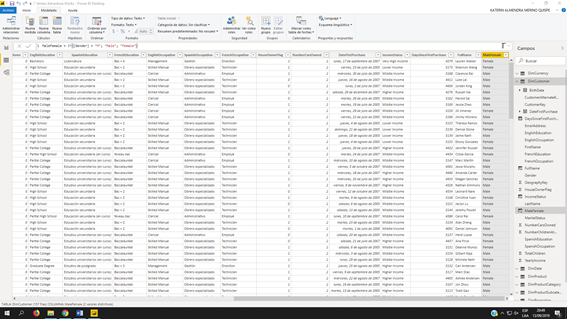
\includegraphics[width=15cm]{./Imagenes/img27} 
\end{center}
\item 15. On the Modeling ribbon, in the Calculations group, click New Column.
\item 16. In the formula bar, highlight Column =, and type:
Relationship = IF([MaritalStatus] = "M", "Married", "Single")
\item 17. Press Enter.

\begin{center}
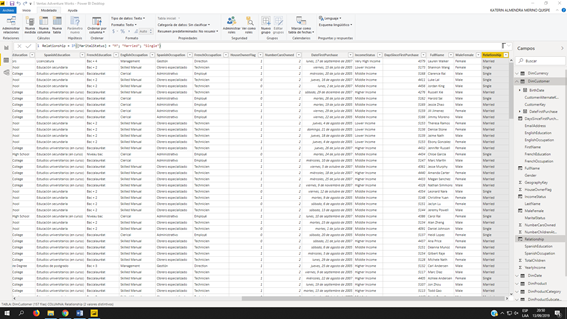
\includegraphics[width=15cm]{./Imagenes/img28} 
\end{center}

\item 18. In the Fields pane, click DimProductSubcategory.
\item 19. On the Modeling ribbon, in the Calculations group, click New Column.
\item 20. In the formula bar, highlight Column =, and type:
MainCategory = RELATED(DimProductCategory[CategoryName])
\item 21. Press Enter

\begin{center}
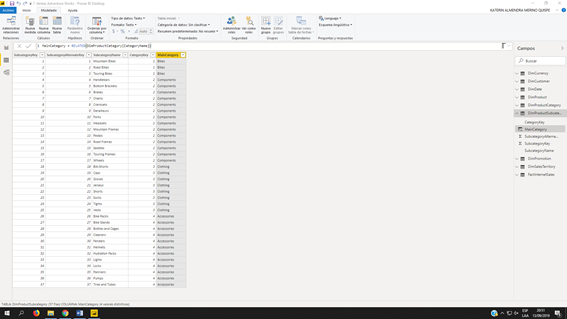
\includegraphics[width=15cm]{./Imagenes/img29} 
\end{center}

\item 22. In the Fields pane, click DimPromotion.
\item 23. On the Modeling ribbon, in the Calculations group, click New Column.
\item 24. In the formula bar, highlight Column =, and type:
PromotionLengthDays = DATEDIFF(DimPromotion[StartDate], DimPromotion[EndDate], DAY)
\item 25. Press Enter.

\begin{center}
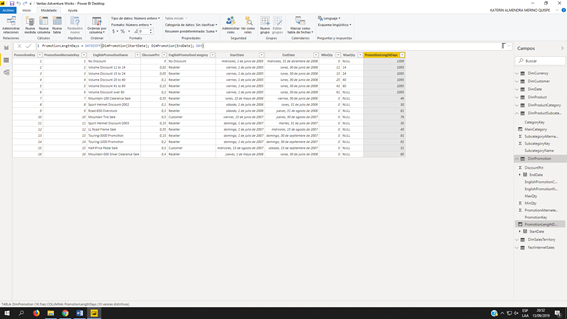
\includegraphics[width=15cm]{./Imagenes/img30} 
\end{center}

\item 26. In the Fields pane, click FactInternetSales.
\item 27. On the Modeling ribbon, in the Calculations group, click New Column.
\item 28. In the formula bar, highlight Column =, and type:
Profit = CURRENCY(FactInternetSales[UnitPrice] -
FactInternetSales[ProductStandardCost])
\item 29. Pressionar Enter.

\begin{center}
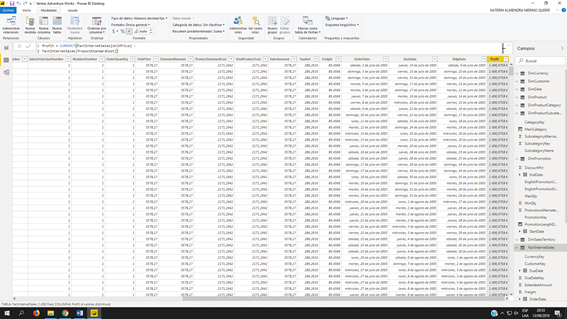
\includegraphics[width=15cm]{./Imagenes/img31} 
\end{center}

\item 30. Cerrar Power BI Desktop, salvando cualquier cambio.


\end{document}
